


We now describe our process for generating FDEs.
Our transformation is reminiscent of the technique of probabilistic tree embeddings~\cite{B96, FRT04, AIK08, CJLW22}, which can be used to transform a set of vectors into a single vector. For instance, they have been used to embed the Earth Mover's Distance into the $\ell_1$ metric~\cite{I04b, AIK08, CJLW22,  jayaram2024data}, and to embed the weight of a Euclidean MST of a set of vectors into the Hamming metric \cite{I04b, jayaram2024massively, 10.1145/3564246.3585168}. However, since we are working with inner products, which are not metrics, instead of $\ell_p$ distances, an alternative approach for our transformation will be needed.


 The intuition behind our transformation is as follows. Hypothetically, for two MV representations $Q,P \subset \R^d$, if we knew the optimal mapping $\pi:Q \to P$ in which to match them, then we could create vectors $\vec{q} ,\vec{p}$ by concatenating all the vectors in $Q$ and their corresponding images in $P$ together, so that $\langle \vec{q},\vec{p}\rangle = \sum_{q \in Q} \langle q, \pi(q) \rangle = \CH(Q,P)$. However, since we do not know $\pi$ in advance, and since different query-document pairs have different optimal mappings, this simple concatenation clearly will not work. Instead, our goal is to find a randomized ordering over \textit{all} the points in $\R^d$ so that, after clustering close points together, the dot product of \textit{any} query-document pair $Q,P \subset \R^d$ concatenated into a single vector under this ordering will approximate the Chamfer similarity. 

The first step is to partition the latent space $\R^d$ into $\buckets$ clusters so that vectors that are closer are more are more likely to land in the same cluster. 
Let $\bvarphi:\R^d \to [\buckets]$ be such a partition; $\bvarphi$ can be implemented via Locality Sensitive Hashing (LSH) \cite{HIM12}, $k$-means, or other methods; we discuss choices for $\bvarphi$ later in this section. After partitioning via $\bvarphi$, the hope is that for each $q \in Q$, the closest $p \in P$ lands in the same cluster (i.e. $\bvarphi(q) = \bvarphi(p)$). Hypothetically, if this were to occur, then:
\begin{equation}\label{eqn:chamfer-ideal}
\CH(Q,P) = \sum_{k=1}^{\buckets} \sum_{\substack{q \in Q \\ \bvarphi(q) = k}} \max_{\substack{p \in P \\ \bvarphi(p)=k}}\langle q,p\rangle
\end{equation}
If $p$ is the only point in $P$ that collides with $q$, then (\ref{eqn:chamfer-ideal}) can be realized as a dot product between two vectors $\vec{q},\vec{p}$ by creating one block of $d$ coordinates in $\vec{q},\vec{p}$ for each cluster $k \in [B]$ (call these blocks $\vec{q}_{(k)},\vec{p}_{(k)} \in \R^{d}$), and setting $\vec{q}_{(k)},\vec{p}_{(k)}$ to be the sum of all $q \in Q$ (resp. $p \in P$) that land in the $k$-th cluster under $\bvarphi$. 
 However, if multiple $p' \in P$ collide with $q$, then $\langle \vec{q}, \vec{p} \rangle$ will differ from (\ref{eqn:chamfer-ideal}), since \emph{every} $p'$ with $\bvarphi(p') = \bvarphi(q)$ will contribute at least $\langle q,p'\rangle$ to $\langle \vec{q}, \vec{p} \rangle$. To resolve this, we set $\vec{p}_{(k)}$ to be the \emph{centroid} of the $p \in P$'s  with $\bvarphi(p) = \bvarphi(q)$. Formally, for $k=1,\dots,\buckets$, we define 
\begin{equation}\label{eqn:define-FDE}
\vec{q}_{(k)}= \sum_{\substack{q \in Q \\ \bvarphi(q) = k}}  q, \qquad \qquad \vec{p}_{(k)} =  \frac{1}{|P \cap \bvarphi^{-1}(k)|} \sum_{\substack{p \in P \\ \bvarphi(p)=k}} p \end{equation}
Setting $\vec{q} =  (\vec{q}_{(1)},\dots,\vec{q}_{(\buckets)})$ and $\vec{p} = (\vec{p}_{(1)},\dots,\vec{p}_{(\buckets)})$, then we have 
\begin{equation}\label{eqn:chamfer-approx}
  \langle \vec{q}, \vec{p} \rangle =   \sum_{k=1}^{\buckets} \sum_{\substack{q \in Q\\ \bvarphi(q) = k}}  \frac{1}{|P \cap \bvarphi^{-1}(k)|} \sum_{\substack{p \in P \\ \bvarphi(p)=k}} \langle q,p\rangle
\end{equation}
Note that the resulting dimension of the vectors $\vec{q},\vec{p}$ is $d  \buckets$. To reduce the dependency on $d$, we can apply a random linear projection $\bpsi:\R^d \to \R^{\dproj}$ to each block $\vec{q}_{(k)},\vec{p}_{(k)}$, where $\dproj < d$. Specifically, we define $\bpsi(x) =(1/ \sqrt{\dproj})S x$, where  $S \in \R^{\dproj \times d}$ is a random matrix with uniformly distributed $\pm 1$ entries. We can then define  $\vec{q}_{(k),\bpsi}= \bpsi(\vec{q}_{(k)})$ and $\vec{p}_{(k),\bpsi}= \bpsi(\vec{p}_{(k)})$, and define the \emph{FDE's with inner projection} as $\vec{q}_{\bpsi} =  (\vec{q}_{(1),\bpsi},\dots,\vec{q}_{(\buckets),\bpsi})$ and $\vec{p}_{\bpsi} = (\vec{p}_{(1),\bpsi},\dots,\vec{p}_{(\buckets),\bpsi})$.  When $d=\dproj$, we simply define $\psi$ to be the identity mapping, in which case $\vec{q}_{\bpsi}, \vec{p}_{\bpsi}$ are identical to $\vec{q}, \vec{p}$. 
To increase accuracy of (\ref{eqn:chamfer-approx}) in approximating (\ref{eqn:chamfer-ideal}), we repeat the above process $\reps \geq 1$ times independently, using different randomized partitions $\bvarphi_1,\dots,\bvarphi_{\reps}$ and projections $\bpsi_1,\dots,\bpsi_{\reps}$. We denote the vectors resulting from $i$-th repetition by $\vec{q}_{i,\bpsi}, \vec{p}_{i,\bpsi}$. Finally, we concatenate these $\reps$ vectors together, so that our final FDEs are defined as $\fdeq(Q) = (\vec{q}_{1,\bpsi},\dots, \vec{q}_{\reps,\bpsi})$ and $\fded(P) = (\vec{p}_{1,\bpsi},\dots, \vec{p}_{\reps,\bpsi})$. 
Observe that a complete FDE mapping is specified by the three parameters $(\buckets, \dproj, \reps)$, resulting in a final dimension of $\dfde =  \buckets \cdot \dproj \cdot \reps $. 


\begin{figure}
    \centering
    \vspace{-2em}
 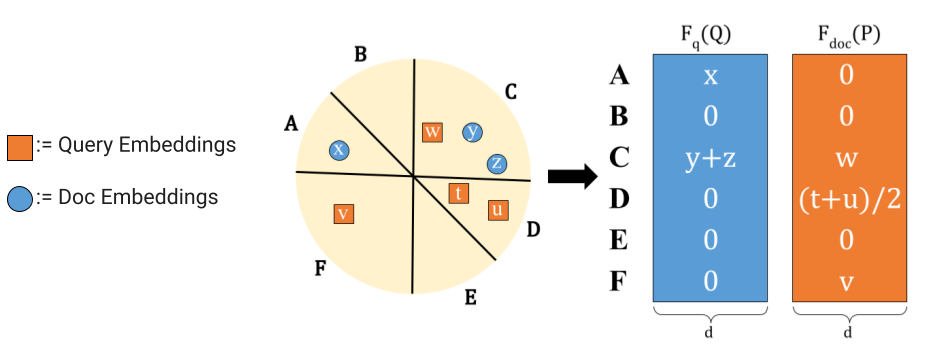
\includegraphics[scale = 0.4]{plots/FDE_with_Labels.png}
    \caption{\small FDE Generation Process. Three SimHashes ($\ksim = 3$) split space into six regions labelled $A$-$F$ (in high-dimensions $B= 2^{\ksim}$, but $B=6$ here since $d=2$). $\fdeq(Q),\fded(P)$ are shown as $B \times d$  matrices, where the $k$-th row is $\vec{q}_{(k)}, \vec{p}_{(k)}$.
   The actual FDEs are flattened versions of these matrices. Not shown: inner projections, repetitions, and \texttt{fill\_empty\_clusters}.}
    \label{fig:FDE}
\end{figure}


\textbf{Choice of Space Partition} When choosing the partition function $\bvarphi$, the desired property is that points are more likely to collide (i.e. $\bvarphi(x)=\bvarphi(y)$) the closer they are to each other. Such functions with this property exist, and are known as \textit{locality-sensitive hash functions} (LSH) (see \cite{HIM12}). When the vectors are normalized, as they are for those produced by ColBERT-style models, SimHash \cite{charikar2002similarity} is the standard choice of LSH. Specifically, for any $\ksim \geq 1$, we sample random Gaussian vectors $g_1,\dots,g_{\ksim} \in \R^d$, and set $\bvarphi(x)= (\mathbf{1}(\langle g_1, x\rangle > 0), \dots,\mathbf{1}(\langle g_{\ksim} , x\rangle> 0) )$, where $\mathbf{1}(\cdot) \in \{0,1\}$ is the indicator function.  Converting the bit-string to decimal, $\bvarphi(x)$ gives a mapping from $\R^d$ to $[\buckets]$ where $\buckets = 2^{\ksim}$. In other words, SimHash partitions $\R^d$ by drawing $\ksim$ random half-spaces, and each of the the $2^{\ksim}$ clusters is formed by the $\ksim$-wise intersection of each of these halfspaces or their complement.
Another natural approach is to choose $k_{\textsc{center}} \geq 1$ centers from the collection of all token embeddings $\cup_{i=1}^n P_i$, either randomly or via $k$-means, and set $\bvarphi(x) \in [k_{\textsc{center}}]$ to be the index of the center nearest to $x$. We compare this method to SimHash in (§\ref{sec:fde-experimental}). 



\textbf{Filling Empty Clusters.} 
A key source of error in the FDE's approximation is when the nearest vector $p \in P$ to a given query embedding $q \in Q$ maps to a different cluster, namely $\bvarphi(p) \neq \bvarphi(q) = k$. This can be made less likely by decreasing $B$, at the cost of making it more likely for other $p' \in P$ to also map to the same cluster, moving the centroid $\vec{p}_{(k)}$ farther from $p$. If we increase $B$ too much, it is possible that no $p \in P$ collides with $\bvarphi(q)$. To avoid this trade-off, we directly ensure that if no $p \in P$ maps to a cluster $k$, then instead of setting $\vec{p}_{(k)} = 0$ we set $\vec{p}_{(k)}$ to the point $p$ that is \emph{closest} to cluster $k$. As a result, increasing $B$ will result in a more accurate estimator, as this results in smaller clusters. 
Formally, for any cluster $k$ with $P \cap \bvarphi^{-1}(k) = \emptyset$, if \texttt{fill\_empty\_clusters} is enabled, we set $\vec{p}_{(k)} = p$ where $p \in P$ is the point for which $\bvarphi(p)$ has the fewest number of disagreeing bits with $k$ (both thought of as binary strings), with ties broken arbitrarily. We do not enable this for query FDEs, as doing so would result in a given $q \in Q$ contributing to the dot product multiple times. 




\textbf{Final Projections.} A natural approach to reducing the dimensionality is to apply a final projection  $\bpsi':\R^{\dfde} \to \R^{\dfinal}$ (also implemented via multiplication by a random $\pm 1$ matrix) to the FDE's, reducing the final dimensionality to any $\dfinal < \dfde$. 
Experimentally, we find that final projections can provides small but non-trivial $1$-$2\%$ recall boosts for a fixed dimension (see  §\ref{app:finalproj}).


\subsection{Theoretical Guarantees for FDEs}
\label{sec:fde-theory}

We now state our theoretical guarantees for our FDE construction. For clarity, we state our results in terms of normalized Chamfer similarity $\nCH(Q,P) = \frac{1}{|Q|}\CH(Q,P)$. This ensures $\nCH(Q,P) \in [-1,1]$ whenever the vectors in $Q,P$ are normalized. Note that this factor of $1/|Q|$ does not affect the relative scoring of documents for a fixed query. 
In what follows, we assume that all token embeddings are normalized (i.e. $\|q\|_2 = \|p\|_2 = 1$ for all $q \in Q, p \in P)$. Note that ColBERT-style late interaction MV models indeed produce normalized token embeddings. We will always use the \texttt{fill\_empty\_clusters} method for document FDEs, but never for queries. 


Our main result is that FDEs give $\eps$-additive approximations of the Chamfer similarity. The proof uses the properties of LSH (SimHash) to show that for each query point $q \in Q$, the point $q$ gets mapped to a cluster $\varphi(q)$ that \emph{only} contains points $p \in P$ that are close to $q$ (within $\eps$ of the closest point to $q$); the fact that at least one point collides with $q$ uses the \texttt{fill\_empty\_partitions} method. 

\begin{theorem}[FDE Approximation]\label{thm:FDE-approx}
Fix any $\eps ,\delta > 0$, and sets $Q,P \subset \R^d$ of unit vectors, and let $m=|Q| + |P|$. 
Then setting $\ksim = O\left(\frac{\log (m\delta^{-1})}{\epsilon}\right)$, $\dproj = O\left(\frac{1}{\eps^2}  \log (\frac{m}{\eps\delta})\right)$, $\reps = 1$, so that $\dfde = (m/\delta)^{O(1/\eps)}$, % so that $\dfde = O(\frac{1}{\eps^2} \cdot (\frac{m}{\delta})^{1/\eps}  \log (\frac{m}{\eps\delta}))$, 
then in expectation and with probability at least $1-\delta$ we have
 \[  \nCH(Q,P)  - \eps \leq \frac{1}{|Q|}\langle \fdeq(Q) , \fded(P) \rangle \leq  \nCH(Q,P) + \eps  \]
\end{theorem}
Finally, we show that our FDE's give an $\eps$-approximate solution to Chamfer similarity search, using FDE dimension that depends only \emph{logarithmically} on the size of the dataset $n$. Using the fact that our query FDEs are sparse (Lemma \ref{lem:runtime}), one can run exact MIPS over the FDEs in time $\tilde{O}(|Q|\cdot n)$, improving on the brute-force runtime of $O(|Q| \max_i|P_i| n)$ for Chamfer similarity search.


\begin{theorem}\label{thm:FDE-ANN}
Fix any $\eps > 0$, query $Q$, and dataset $P = \{P_1,\dots,P_n\}$, where $Q \subset \R^d$ and each $P_i \subset \R^d$ is a set of unit vectors. Let $m=|Q| + \max_{i \in [n]}|P_i|$. 
Let $\ksim = O(\frac{\log m}{\epsilon})$, $\dproj = O(\frac{1}{\eps^2} \log (m/\eps))$ and $\reps = O(\frac{1}{\eps^2}\log n)$ so that $\dfde =  m^{O(1/\eps)} \cdot  \log n$. Then if $i^* = \arg \max_{i \in [n]}\langle \fdeq(Q) , \fded(P_i) \rangle$, with high probability (i.e. $1-1/\poly(n)$) we have:
\[ \nCH(Q,P_{i^*}) \geq \max_{i \in [n]} \nCH(Q,P_i) - \eps \]
Given the query $Q$, the document $P^*$ can be recovered in time $O\left(|Q| \max\{d,n\}  \frac{1}{\eps^4} \log(\frac{m}{\eps}) \log n \right)$. 
\end{theorem}












\section{Evaluation} \label{sec:eval}
In this section, we evaluate our FDEs as a method for MV retrieval. First, we evaluate the FDEs themselves (offline) as a proxy for Chamfer similarity (§\ref{sec:fde-experimental}). In (§\ref{sec:online}), we discuss the implementation of $\name$, as well as several optimizations made in the search. Then we evaluate the latency of $\name$ compared to PLAID, and study the effects of the aforementioned optimizations.



\textbf{Datasets.} Our evaluation includes results from six of the well-studied BEIR \cite{thakur2021beir} information retrieval datasets: MS MARCO \cite{nguyen2016ms} (CC BY-SA 4.0), HotpotQA (CC BY-SA 4.0) \cite{yang2018hotpotqa}, NQ (Apache-2.0) \cite{kwiatkowski2019natural}, Quora (Apache-2.0) \cite{thakur2021beir}, SciDocs (CC BY 4.0) \cite{cohan2020specter}, and ArguAna (Apache-2.0) \cite{wachsmuth2018retrieval}. These datasets were selected for varying corpus size (8K-8.8M) and average number of document tokens (18-165); see (§\ref{app:datasets}) for further dataset statistics. Following \cite{santhanam2022plaid}, we use the development set for our experiments on MS MARCO, and use the test set on the other datasets.  


\textbf{MV Model, MV Embedding Sizes, and FDE Dimensionality.}
We compute our FDEs on the MV embeddings produced by the ColBERTv2 model \cite{santhanam2021colbertv2} (MIT License), which have a dimension of $d= 128$ and a fixed number $|Q|=32$ of embeddings per query. The number of document embeddings is variable, ranging from an average of $18.3$ on Quora to $~165$ on Scidocs. This results in ~2,300-21,000 floats per document on average (e.g. 10,087 for MS MARCO). Thus, when constructing our FDEs we consider a comparable range of dimensions $\dfde$ between ~1,000-20,000. Furthermore,  using product quantization, we show in (§\ref{sec:online}) that the FDEs can be significantly compressed by $32\times$ with minimal quality loss, further increasing the practicality of FDEs.  


\subsection{Offline Evaluation of FDE Quality}
\label{sec:fde-experimental}
We evaluate the quality of our FDEs as a proxy for the Chamfer similarity, without any re-ranking and using exact (offline) search. We first demonstrate that FDE recall quality improves dependably as the dimension $\dfde$ increases, making our method relatively easy to tune. We then show that FDEs are a more effective method of retrieval than the SV heuristic. Specifically, the FDE method achieves Recall$@N$ exceeding the Recall$@$2-4N of the SV heuristic, while in principle scanning a similar number of floats in the search. This suggests that the success of the SV heuristic is largely due to the significant effort put towards optimizing it (as supported by \cite{macavaney2024reproducibility}), and similar effort for FDEs may result in even bigger efficiency gains. Additional plots can be found in (§\ref{sec:additional-plots}). All recall curves use a single FDE instantiation, since in (§\ref{app:variance}) we show the variance of FDE recall is negligible. 



\textbf{FDE Quality vs. Dimensionality.}
We study how the retrieval quality of FDE's improves as a function of the dimension $\dfde$. We perform a grid search over FDE parameters $\reps \in \{1,5,10,15,20\}, \ksim \in \{2,3,4,5,6\}, \dproj \in \{8,16,32,64\}$, and compute recall on MS MARCO (Figure \ref{fig:grid_search}). We find that Pareto optimal parameters are generally achieved by larger $\reps$, with $\ksim,\dproj$ playing a lesser role in improving quality. Specifically, $(\reps,\ksim,\dproj) \in\{ (20,3,8),(20,4,8)(20,5,8),(20,5,16) \}$ were all Pareto optimal for their respective dimensions (namely $\reps \cdot 2^{\ksim} \cdot \dproj$).
While there are small variations depending on the parameter choice, the FDE quality is tightly linked to dimensionality; increase in dimensionality will generally result in quality gains. 
We also evaluate using $k$-means as a method of partitioning instead of SimHash. Specifically, we cluster the document embeddings with $k$-means and set $\varphi(x)$ to be the index of the nearest centroid to $x$. We perform a grid search over the same parameters (but with $k \in \{4,8,16,32,64\}$ to match $B = 2^{\ksim}$). We find that $k$-means partitioning offers no quality gains on the Pareto Frontier over SimHash, and is often worse.  Moreover, FDE construction with $k$-means is no longer data oblivious. 
Thus, SimHash is chosen as the preferred method for partitioning for the remainder of our experiments. 



\begin{figure}[t]
    \centering
 %   \vspace{-2em}
  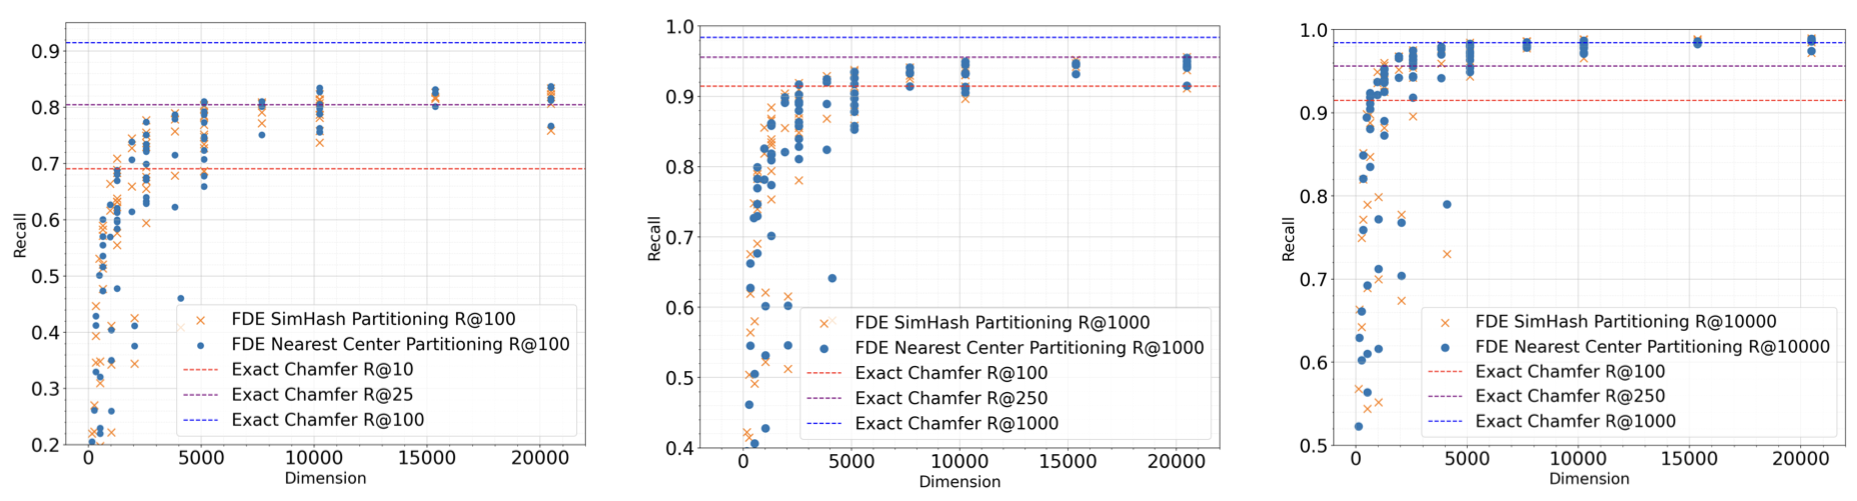
\includegraphics[width=\linewidth]{plots/Grid_Search_Three.png}
    \caption{\small FDE recall vs dimension for varying FDE parameters on MS MARCO. Plots show FDE Recall$@$100,1k,10k left to right.  Recalls$@N$ for exact Chamfer scoring is shown by dotted lines. }
         \label{fig:grid_search} % Add a label (optional)
\end{figure}


\begin{figure}[t]
    \centering
   % \vspace{-1em}
  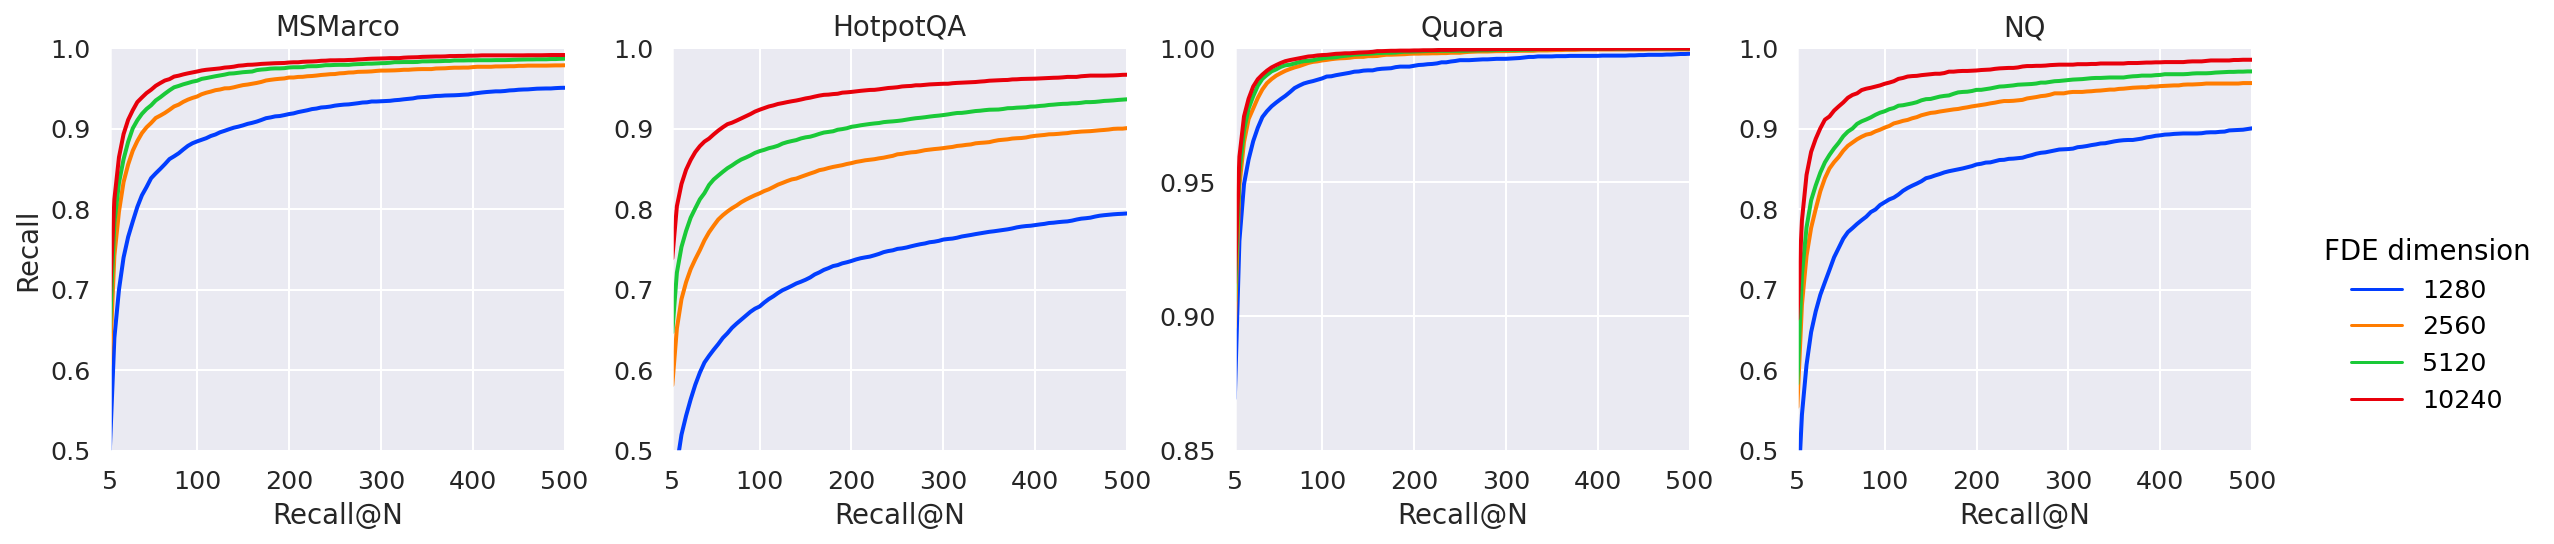
\includegraphics[width=\linewidth]{plots/recall_vs_chamfer.png}
    \caption{\small Comparison of FDE recall versus brute-force search over Chamfer similarity.}
         \label{fig:chamfer} % Add a label (optional)
\end{figure}



In Figure \ref{fig:chamfer}, we evaluate the FDE retrieval quality with respect to the Chamfer similarity (instead of labelled ground truth data).  We compute $1$Recall@$N$, which is the fraction of queries for which the Chamfer $1$-nearest neighbor is among the top-$N$ most similar in FDE dot product. We choose FDE parameters which are Pareto optimal for the dimension from the above grid search. We find that FDE's with fewer dimensions that the original MV representations achieve significantly good recall across multiple BEIR retrieval datasets. For instance, on MS MARCO (where $d\cdot m_{avg} \approx 10K$) we achieve $95\%$ recall while retrieving only $75$ candidates using $\dfde = 5120$.


\paragraph{Single Vector Heuristic vs. FDE retrieval.}
We compare the quality of FDEs as a proxy for retrieval against the previously described SV heuristic, which is the method underpinning PLAID.
Recall that in this method, for each of the $i=1,\dots,32$ query vectors $q_i$ we compute the $k$ nearest neighbors $p_{1,i},\dots,p_{k,i}$ from the set $\cup_{i} P_i$ of all documents token embeddings. To compute Recall$@N$, 
%we collect the relevant document ID's $\ell_{1,i},\dots,\ell_{k,i}$, 
we create an ordered list $\ell_{1,1},\dots,\ell_{1,32}, \ell_{2,1},\dots$, where $\ell_{i,j}$ is the document ID containing $p_{i,j}$, consisting of the $1$-nearest neighbors of the queries, then the $2$-nearest neighbors, and so on. When re-ranking, one firsts removes duplicate document IDs from this list. Since duplicates cannot be detected while performing the initial $32$ SV MIPS queries, the SV heuristic needs to over-retrieve to reach a desired number of unique candidates. Thus, we note that the true recall curve of implementations of the SV heuristic (e.g. PLAID) is somewhere between the case of no deduplication and full deduplication; we compare to both in Figure \ref{fig:sv_mv}. 

 

To compare the cost of the SV heuristic to running MIPS over the FDEs, we consider the total number of floats scanned by both using a brute force search. 
The FDE method must scan $n\cdot \dfde$ floats to compute the $k$-nearest neighbors. For the SV heuristic, one runs $32$ brute force scans over $n\cdot m_{avg}$ vectors in $128$ dimensions, where $m_{avg}$ is the average number  embeddings per document (see §\ref{app:datasets} for values of $m_{avg}$). For MS MARCO, where $m_{avg} = 78.8$, the SV heuristic searches through $32 \cdot 128 \cdot 78.8 \cdot n$ floats. This allows for an FDE dimension of $\dfde =$ 322,764 to have comparable cost! We can extend this comparison to fast approximate search -- suppose that approximate MIPS over $n$ vectors can be accomplished in sublinear $n^\eps$ time, for some $\eps \in (0,1)$. Then even in the unrealistic case of $\eps=0$, we can still afford an FDE dimension of $\dfde = 32\cdot 128 = 4096$.

The results can be found in Figure \ref{fig:sv_mv}. We build FDEs once for each dimension, using $\reps = 40, \ksim = 6, \dproj = d = 128$, and then applying a final projection to reduce to the target dimension (see \ref{app:finalproj} for experiments on the impact of final projections).
On MS MARCO, even the $4096$-dimensional FDEs match the recall of the (deduplicated) SV heuristic while retrieving 1.75-3.75$\times$ \emph{fewer} candidates  (our Recall$@N$ matches the Recall$@$1.75-3.75$N$ of the SV heuristic), and 10.5-15$\times$ fewer than to the non-deduplicated SV heuristic. For our $10240$-dimension FDEs, these numbers are 2.6-5$\times$ and 20-22.5$\times$ fewer, respectively. For instance, we achieve $80\%$ recall with $60$ candidates when $\dfde = 10240$ and $80$ candidates when $\dfde = 4096$, but the SV heuristic requires $300$ and $1200$ candidates (for dedup and non-dedup respectively). See Table \ref{table:sv_mv_table} for further comparisons.



\begin{figure}[t]
    \centering
   % \vspace{-1.5em}
  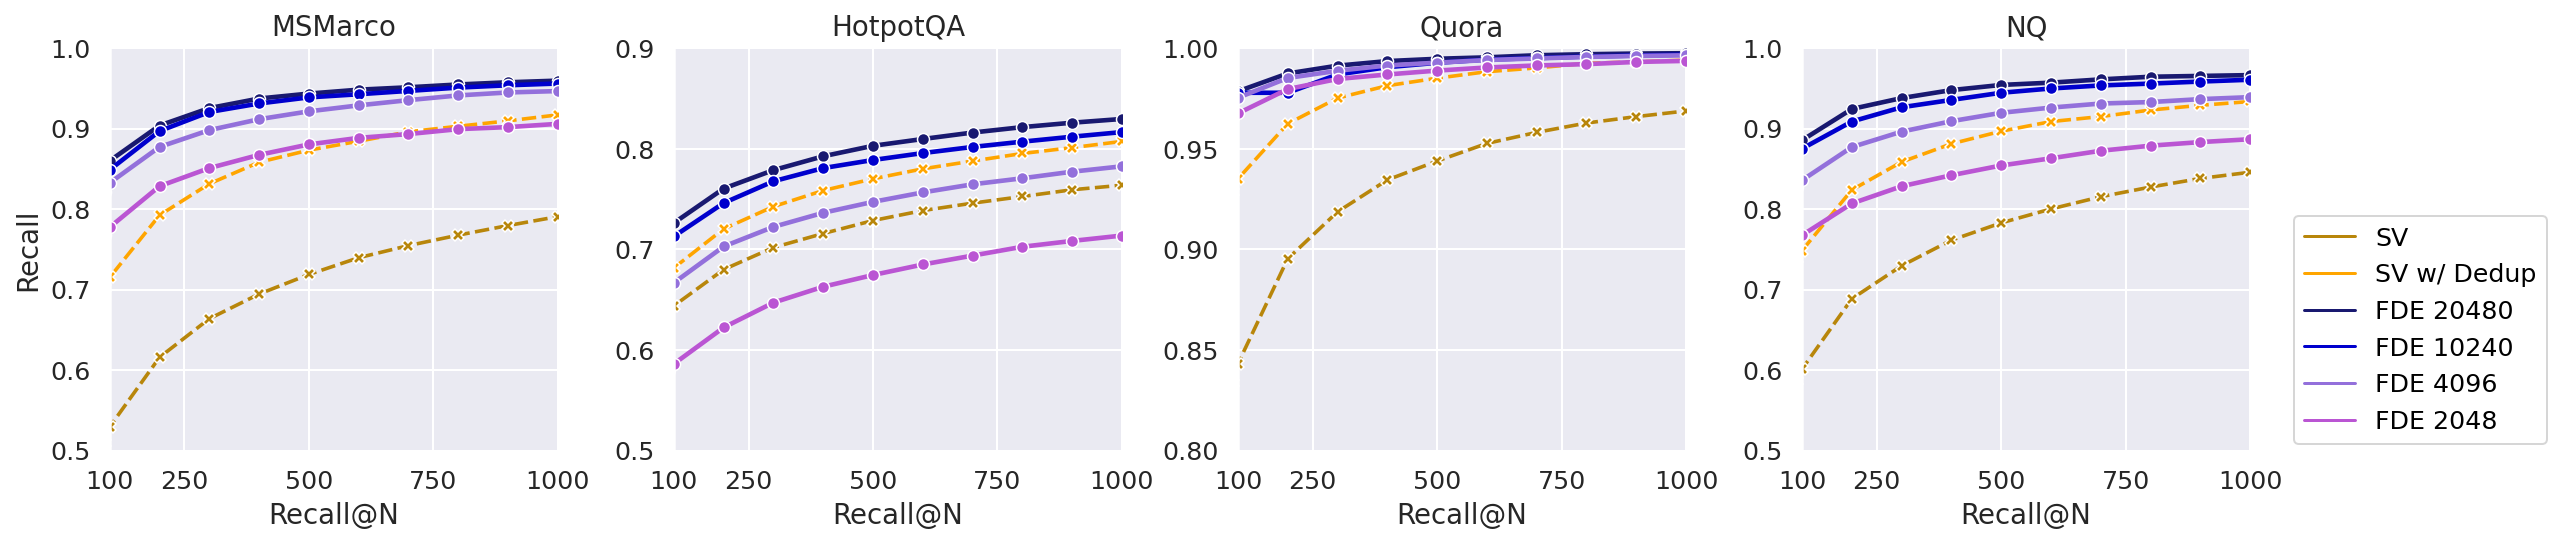
\includegraphics[width=\linewidth]{plots/SV_vs_MV.png}
   \caption{\small FDE retrieval vs SV Heuristic, both with and without document id deduplication. }
         \label{fig:sv_mv} % Add a label (optional)
\end{figure}




\paragraph{Variance.}Note that although the FDE generation is a randomized process, we show in (§\ref{app:variance}) that the variance of the FDE Recall is essentially negligible; for instance, the standard deviation Recall$@$1000 is at most $0.08$-$0.16\%$ for FDEs with $2$-$10k$ dimensions.

